\section{Approach} 

There are countless different approaches one could take to calibrate a camera, 



however they all build upon techniques first described in multiple highly influential papers, most notably Tsai's ``A Versatile Camera Calibration Technique for High-Accuracy 3D Machine Vision Metrology Using Off-the-shelf TV Cameras and Lenses'' and Zhang's ``A Flexible New Technique for Camera Calibration''. 
\subsection{Camera Model} \label{sec:camera_model}

A camera model is a projection model which approximates the function of a camera by describing a mathematical relationship between points in 3D space and its projection onto the sensor grid of the camera. In order to construct such a model, we must first understand the general workings of a camera.

The modern lens Camera is highly sophisticated, built with an array of complex mechanisms and a wide range of features. The complexity of cameras can be better understood simplifying the lens camera into three main elements critical to image projection: the lens, the aperture, and the sensor grid (CCD). 

\begin{itemize}[leftmargin=!, itemindent=-5ex]
    \item Lens -- Focuses incoming light rays and projects it onto the sensor grid. Modern cameras have compound lenses (lenses made up of several lens elements) in order to minimize undesired effects such as aberration, blurriness, and distortion. 
    \item Aperture -- Controls the amount of light that reaches the sensor. By adjusting the aperture size, the exposure and depth of field can be modified.
    \item Sensor Grid -- Captures the projected image created by the lens and the aperture. 
\end{itemize}

\begin{figure}[H]
    \centering
    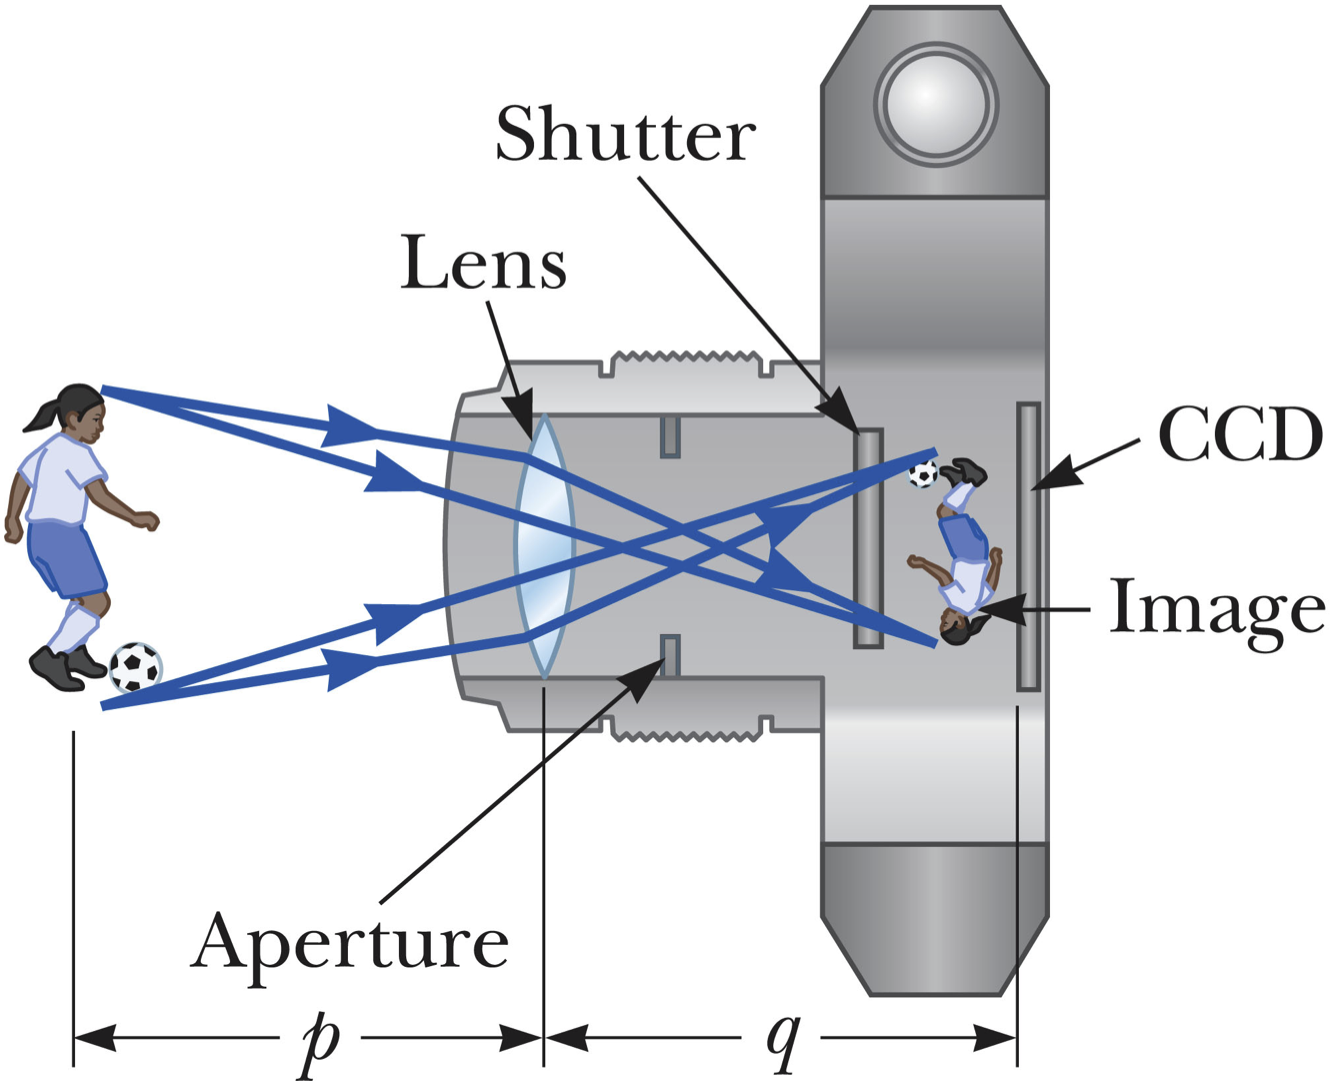
\includegraphics[width=0.5\textwidth]{images/lens_camera}
    \caption{Lens camera. Adapted from \cite{coltonPhysics1232012}} \label{fig:lens_camera}
\end{figure}

However, even a simplified model of a lens camera is still too complicated to describe, as it is impossible to encapsulate the complex behavior of a lens using a simple mathematical equation. As such, we need to sacrifice some precision by find a simpler model which sufficiently describes the behavior of a lens camera. 

\subsubsection{Pinhole Camera Model}

A pinhole camera is a simple camera without a lens. Instead, it relies on the use of a tiny hole as the aperture of the camera, and light rays pass through the hole, projecting an inverted image onto the image plane. The pinhole camera model is based on the pinhole camera, however it goes further by making a few important assumptions for the purpose of simplification:

\begin{enumerate}[leftmargin=!, itemindent=-5ex]
    \item \textbf{The aperture is infinitely small} -- This means that any incoming light ray can only travel straight through the pinhole, and that a point in space can only map to one single point on image plane. This allows us to establish a relationship between a 3D point and its 2D projection onto the image plane. 
    \item \textbf{Infinite depth of field} -- 
\end{enumerate}
 

\begin{figure}
    \centering
    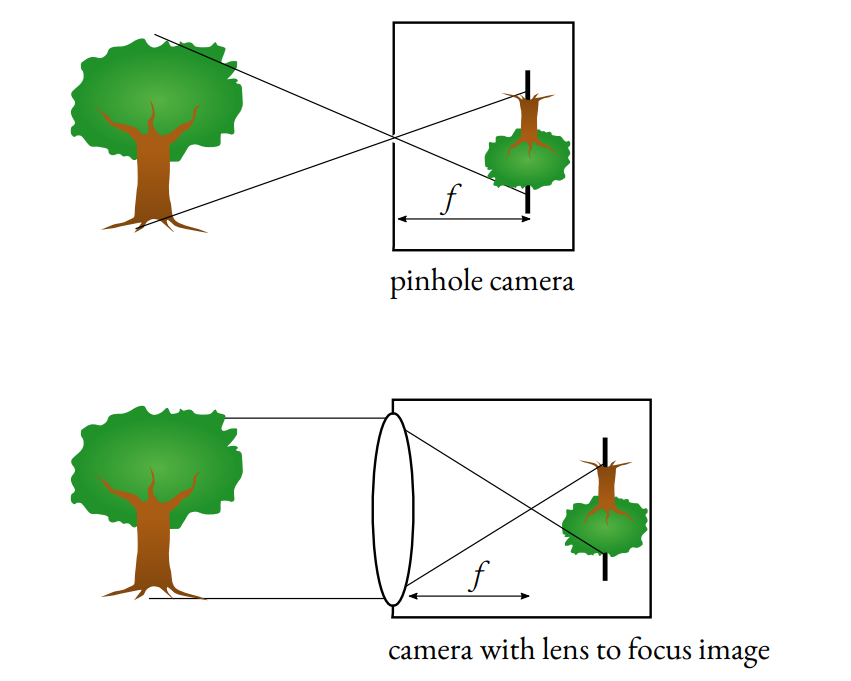
\includegraphics[width=0.7\textwidth]{images/pinhole_vs_lens}
    \caption{Difference between a pinhole camera and a lens camera. Adapted from \cite{leCameraModel2018}}
\end{figure}


Extremely simple model for imaging geometry
Doesn't strictly apply
Mathematically convenient acceptable approximation.


While the pinhole camera model is an extremely basic  model that does not accurately describe the true behavior of cameras, it is extremely simple. As such, for the sake of simplifying camera models, the pinhole camera model is often used. This model is one of the most basic and frequently employed camera models in the field of camera calibration. 

\begin{itemize}[leftmargin=!, itemindent=-4ex]
    \item \textbf{3D} -- 
    \item \textbf{2D} -- 
    \item \textbf{1D} -- 
\end{itemize}







\subsection{Calibration Object}

Calibration techniques can be roughly separated into 3 categories, based on the dimension of the calibration object used \footcite{zhangCameraCalibration2007}:

